% \newpage
\section*{Задание 7: Структурированное извлечение данных из изображений}
\subsection{Постановка задачи}
\noindent
Тип входного изображения: Фотография ценников на полке магазина \\
Сущности для извлечения: Название продукта, Цена за единицу, Скидка (если есть), Штрих-код (цифры) \\
Сложность / Шум: Множество объектов в кадре, блики на ценникодержателях \\
Целевая структура JSON: \{"products": {[} \{"name": string, "price": float, \\ "discount\_percent": int\_or\_null\} {]} \} \\
\newline
Исходное изображение – фотография, сделанная в супермаркете: на полке выстроены упаковки товаров, перед каждой – распечатанный ценник. На ценниках – название, цена, мелкий штрих-код.
\begin{figure}[H]
	\centering
	
\includegraphics[width=17cm]{z7/0.jpg}
	\caption{Пример для промптинга}
\end{figure}
\subsection{Гипотеза и декомпозиция}
Для успешного извлечения данных необходимо:
\begin{itemize}
	\item заставить модель строго следовать JSON-схеме;
	\item применить Chain-of-Thought для пошагового анализа;
	\item явно обработать отсутствие скидки (значение null) и неразборчивые ценники (опустить или отметить как null);
	\item предусмотреть борьбу с галлюцинациями (например, не придумывать товары, которых нет на фото).
\end{itemize}
Базовый подход: дать модели роль «высокоточного OCR-ассистента», затем попросить сначала перечислить все найденные ценники (текст, цифры), а потом структурировать их.
\newpage
\subsection{Журнал генерации и отладки}
\indent \textbf{Итерация 1} \\
Промпт v1:
\textit{«Опиши все ценники на этой фотографии и выведи данные в формате JSON: название товара, цена, скидка, штрих-код.»} \\
\newline
Результат:
\begin{figure}[H]
	\centering
	
\includegraphics[width=15cm]{z7/1b.png}
	\caption{Итерация 1, модель (b)}
\end{figure}
\newpage
\begin{figure}[H]
	\centering
	
\includegraphics[width=17cm]{z7/1a.png}
	\caption{Итерация 1, модель (a)}
\end{figure}
\indent \textbf{Анализ ошибок:} \\
Модель добавила штрих-коды, которых на фото не было видно (галлюцинация).
Некоторые цены считаны неправильно (на фото слева ценник обрезан и цена 123 была прочитана как 23).
Скидку не всегда верно находит.
Не указано, что штрих-коды были нечитаемы.\\
\newline
\indent \textbf{Корректировка:} \\
Добавить запрет на выдумывание цифр, потребовать сначала распознать текст «как есть», а только потом парсить.
\newpage
\indent \textbf{Итерация 2} \\
Промпт v2: \textit{«Ты – точная OCR-система. Сначала внимательно рассмотри фотографию и выпиши в свободной форме всё, что видишь на каждом ценнике: название, цену, процент скидки, цифры штрих-кода (если они различимы). Не придумывай данные, если цифры нечитаемы. Затем преобразуй этот список в JSON по схеме: \{"products": {[}\{"name": string, "price": float, "discount\_percent": int\_or\_null\}{]}\}. Штрих-коды в JSON не включай, они нужны только для проверки. Выведи только JSON, без пояснений.»} \\
\newline
Результат:
\begin{figure}[H]
	\centering
	
\includegraphics[width=15cm]{z7/2b.png}
	\caption{Итерация 2, модель (b)}
\end{figure}
% \newpage
\begin{figure}[H]
	\centering
	
\includegraphics[width=17cm]{z7/2a.png}
	\caption{Итерация 2, модель (a)}
\end{figure}
\newpage
\indent \textbf{Анализ ошибок:} \\
Модель уже не галлюцинирует штрих-коды.
Названия извлечены корректно.
Однако на фото было 2 ценника, но модель вернула только один (второй обрезан).
Модель посчитала скидку на одном ценнике, от цены другого ценника. \\
\newline
\indent \textbf{Корректировка:} \\
Указать, что нужно рассматривать каждый ценник отдельно и не <<вычислять>> скидку а просто записать как есть. Также усилить обработку бликов. \\
\newline
\indent \textbf{Итерация 3} \\
Промпт v3:
\textit{«Ты – профессиональный OCR-инструмент с функцией извлечения структурированных данных.
Перед тобой фотография полки магазина. На полке несколько ценников, некоторые частично скрыты бликами.
Последовательно перебери все видимые ценники (не пропускай ни одного). Для каждого укажи:
название товара (текст),
цену (число в рублях),
скидку (процент если на ценнике напрямую указано, иначе null, вычислять самостоятельно не нужно)
Если какой-то параметр не удаётся прочитать из‑за блика, размытия или угла съёмки, поставь null.
После этого сформируй JSON строго по схеме \{"products": {[}\{"name": string, "price": float, "discount\_percent": int\_or\_null\}{]}\}.
Не добавляй штрих-коды в JSON.
Выведи только JSON, без лишнего текста.»} \\
\newline
Результат:
\begin{figure}[H]
	\centering
	
\includegraphics[width=17cm]{z7/3a.png}
	\caption{Итерация 3, модель (a)}
\end{figure}
\newpage
\begin{figure}[H]
	\centering
	
\includegraphics[width=15cm]{z7/3b.png}
	\caption{Итерация 3, модель (b)}
\end{figure}
На левом ценнике модель не может точно сказать какая там цена, так как ценник обрезан, на том ценнике видна только ценна без скидки.
Также можно сказать, что фактически там есть скидка, в размере 13\% но модель её не может посчитать, потому что не знает цену наверняка и также это ограничено в промпте.
\subsection{Визуализация результатов}
\begin{figure}[H]
	\centering
	
\includegraphics[width=17cm]{z7/1.jpg}
	\caption{Изображение 1}
\end{figure}
Ответ модели (a):
\begin{verbatim}
{"products":[{"name":"Яблоки Гольден","price":79,"discount_percent":
null},{"name":"Яблоки Гольден","price":79,"discount_percent":null},
{"name":"Яблоки Ред Делишес","price":79,"discount_percent":null},{
"name":"Яблоки Бребурн","price":69,"discount_percent":null},{"name":
"Яблоки Гренни Смит","price":69,"discount_percent":null},{"name":
"Яблоки Гренни Смит","price":69,"discount_percent":null},{"name":
"Груши Конференц","price":79,"discount_percent":null},{"name":
"Груши Аббат","price":89,"discount_percent":null},{"name":
"Груши Китайские","price":59,"discount_percent":null}]}
\end{verbatim}
\newpage
\begin{figure}[H]
	\centering
	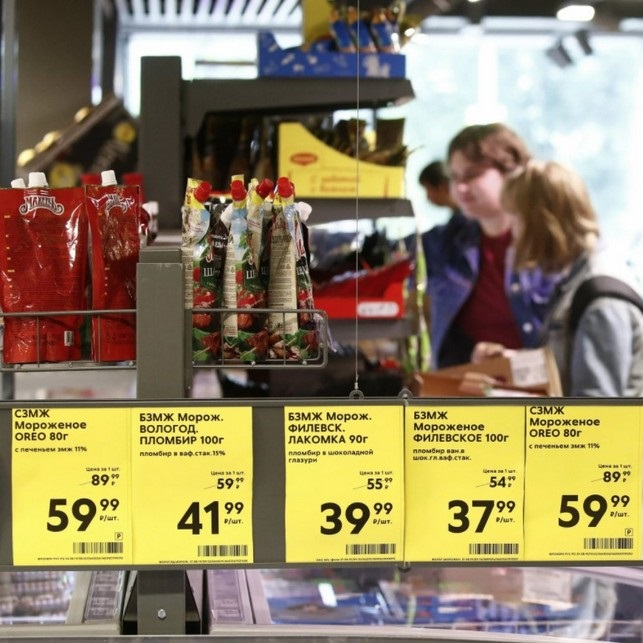
\includegraphics[width=17cm]{z7/2.jpg}
	\caption{Изображение 2}
\end{figure}
\begin{verbatim}
{"products":[{"name":"СЗМЖ Мороженое OREO 80г","price":59.99,
"discount_percent":11},{"name":"БЗМЖ Морож. ВОЛОГОД. ПЛОМБИР 100г",
"price":41.99,"discount_percent":null},{"name":"БЗМЖ Морож. ФИЛЕВСК. 
ЛАКОМКА 90г","price":39.99,"discount_percent":null},{"name":
"БЗМЖ Мороженое ФИЛЕВСКОЕ 100г","price":37.99,"discount_percent":null},
{"name":"СЗМЖ Мороженое OREO 80г","price":59.99,"discount_percent":11}]}
\end{verbatim}
\newpage
\begin{figure}[H]
	\centering
	
\includegraphics[width=17cm]{z7/3.png}
	\caption{Изображение 3}
\end{figure}
\begin{verbatim}
{"products":[{"name":"Сосиски ПАПА МОЖЕТ ВЕНСКИЕ 450г","price":219.99,
"discount_percent":null},{"name":
"СОСИСКИ СТАРОДВОРЬЕ 450г МОЛОЧНЫЕ ПО-СТАРОДВОРСКИ","price":159.99,
"discount_percent":null},{"name":"Сосиски СЕЛО ЗЕЛЕНОЕ ДОРОЖНЫЕ 400г",
"price":95.99,"discount_percent":null}]}
\end{verbatim}
\newpage
\begin{figure}[H]
	\centering
	
\includegraphics[width=17cm]{z7/4.png}
	\caption{Изображение 4}
\end{figure}
\begin{verbatim}
{"products":[{"name":"Кета РРК филе с кожей 500г","price":219.99,
"discount_percent":null},{"name":"FISH HOUSE","price":179.99,
"discount_percent":null},{"name":"Мойва HOUSE","price":109.99,
"discount_percent":null},{"name":"Камбала МОРЕПРОДУКТ 800г",
"price":69.99,"discount_percent":null},{"name":
"Кальмар FISH HOUSE 800г","price":179.99,"discount_percent":null},
{"name":"Окунь морской FISH HOUSE 800г","price":309.99,
"discount_percent":null}]}
\end{verbatim}
\newpage
\subsection{Сравнение моделей}
\begin{table}[h!]
	\centering
	\begin{tabular}{|l|p{5cm}|p{5cm}|}
		\hline
		\textbf{Критерий} & \textbf{модель (a)} & \textbf{модель (b)} \\
		\hline
		Полнота извлечения \\(кол-во найденных ценников) & 4 & 6 \\
		\hline
		Точность названий & 4 & 5 \\
		\hline
		Точность цен & 4 & 6 \\
		\hline
		Обработка скидок  & 3 & 3 \\
		\hline
		Соблюдение JSON-схемы & 5 & 5 \\
		\hline
		Галлюцинации & Немного & Нет \\
		\hline
		\textbf{Итог} & 3.5 & 5\\
		\hline
	\end{tabular}
\end{table}
Как показала практика, модель (b) очень хорошо распознаёт ценники, а именно: перекрытые ценники, обрезанные ценники, ценники с бликами. Эта модель хорошо <<достраивает>> изображение в обработке. Также эта модель хорошо определяет перекрытые ценники (через просвет) и даже полностью перекрытые (по контексту).
На счёт модели (a) можно сказать, что она тоже справляется с основной задачей, но менее феерично.
\subsection{Финальный промпт}
\textit{«Ты – профессиональный OCR-инструмент с функцией извлечения структурированных данных.
Перед тобой фотография полки магазина. На полке несколько ценников, некоторые частично скрыты бликами.
Последовательно перебери все видимые ценники (не пропускай ни одного). Для каждого укажи:
название товара (текст),
цену (число в рублях),
скидку (процент если на ценнике напрямую указано, иначе null, вычислять самостоятельно не нужно)
Если какой-то параметр не удаётся прочитать из‑за блика, размытия или угла съёмки, поставь null.
После этого сформируй JSON строго по схеме \{"products": {[}\{"name": string, "price": float, "discount\_percent": int\_or\_null\}{]}\}.
Не добавляй штрих-коды в JSON.
Выведи только JSON, без лишнего текста.»}
\newpage
\subsection{Вывод}
\begin{itemize}
	\item Применение Chain-of-Thought (пошаговое перечисление перед формированием JSON) существенно снизило количество галлюцинаций и пропусков.
	\item Чёткое описание правил для нечитаемых данных (использование null) повысило надёжность пайплайна.
	\item Промпт-инжиниринг позволил компенсировать отсутствие тонкой настройки гиперпараметров у моделей с закрытым кодом.
	\item Наибольшую сложность представляла обработка бликов и множества объектов; справиться с этим помогла инструкция "перебери все ценники, даже если часть данных нечитаема".
\end{itemize}